\documentclass[14pt]{article}

\usepackage[margin=3cm]{geometry}
\usepackage{fancyvrb}
\usepackage{fancyhdr}
\usepackage{lastpage}
\usepackage{tcolorbox}
\usepackage{multirow}
\usepackage{float} 
\usepackage{tabularx}
\usepackage[colorlinks = true,
            linkcolor = black,
            urlcolor  = blue,
            citecolor = blue,
            anchorcolor = blue]{hyperref}
\renewcommand{\contentsname}{Indice}

% STEP 1: include the package
\usepackage{img/uninaFrontespizio}

\begin{document}

\pagestyle{fancy}
\cfoot{}
\lhead{Ratatouille23}
\rhead{Gruppo: INGSW2223\_N\_46}
\lfoot{Paolo Cammardella}
\rfoot{Pagina \thepage \ di \pageref{LastPage}}
\renewcommand{\figurename}{}
\renewcommand{\thefigure}{M\arabic{figure}}
\setcounter{section}{-1}
% STEP 2: Front-page configuration
\Universita{Università degli Studi di Napoli Federico II}
\Facolta{Scuola Politecnica e delle Scienze di Base}
\Dipartimento{Dipartimento di Ingegneria Elettrica e Tecnologie dell'Informazione}
\CorsoDiLaurea{Corso di Laurea Magistrale in Informatica}
\Materia{Ingegneria del software} % optional
\AnnoAccademico{Anno Accademico 2022--2023}
\Titolo{Ratatouille23}
\Relatore{S. D. \textsc{Martino}}
\Relatore{F. \textsc{cutugno}}
\Relatore{L. L. L. \textsc{starace}}
\Relatore{M. \textsc{grazioso}}
% can add as many "Relatori" as you wish
\RelatoreLabel{Professori} %optional, default: Relatore
%\relandcorrelsep{2em} %optional, vertical space between relatori and correlatori default: 1.5ex

%\Correlatore{Dott.Foo \textsc{Bar}} % can add as many "Correlatori" as you wish
\CorrelatoreLabel{} %optional, default: Correlatore
\Candidato{Paolo \textsc{Cammardella}} %only one candidate is currently supported
\Matricola{N86/3043}
\Logo{img/logo-federico-II.pdf} %path to logo image
\LogoWidth{3.5cm} %optional, default: 3cm
\LogoPosition{below-uni} % or top, or below-title, or above-title, or no-logo
% STEP 3: use \makefrontpage and/or \makefrontpagealt
\makefrontpage
\tableofcontents
\section{Glossario}
Qui sono racchiuse tutte le definizioni e gli acronimi che sono stati  utilizzati nella documentazione.
\subsection{Definizioni}

\paragraph{Scalabilità} si riferisce alla capacità di un sistema di aumentare o diminuire le risorse a seconda delle necessità.

\paragraph{Usabilità} l'usabilità di un prodotto è il grado con cui esso può essere usato da specificati utenti per
raggiungere specificati obiettivi con efficacia, efficienza e soddisfazione in uno specificato
contesto d'uso.
\paragraph{Mock-up} Un mock-up, è una realizzazione a scopo illustrativo o meramente espositivo di un oggetto o un sistema, senza le complete funzioni dell'originale. Un mockup può rappresentare la totalità o solo una parte dell'originale di riferimento (già esistente o in fase di progetto), essere in scala reale oppure variata.

\paragraph{Class diagram} I class diagram (diagrammi delle classi, in italiano) sono uno dei tipi di diagrammi che possono comparire in un modello UML.
\\
In termini generali, consentono di descrivere tipi di entità, con le loro caratteristiche e le eventuali relazioni fra questi tipi. Gli strumenti concettuali utilizzati sono il concetto di classe del paradigma object-oriented e altri correlati.
\paragraph{Sequenc diagram} Un Sequence Diagram (Diagramma di sequenza, in italiano) è un diagramma previsto dall'UML utilizzato per descrivere uno scenario.

\paragraph{Scenario} Uno scenario è una determinata sequenza di azioni in cui tutte le scelte sono state già effettuate; in pratica nel diagramma non compaiono scelte, né flussi alternativi.

\paragraph{State chart diagram} Uno state chart (diagramma di stato, in italiano) è un tipo di diagramma usato in informatica per descrivere il comportamento dei sistemi, il quale viene analizzato e rappresentato tramite una serie di eventi che potrebbero accadere per ciascuno stato. Per poter essere realizzato, il sistema deve essere composto da un numero finito di stati.

\paragraph{Activity diagram} Un activity diagram (diagramma di attività in italiano) è un tipo di diagramma che permette di descrivere un processo attraverso dei grafi in cui i nodi rappresentano le attività e gli archi l'ordine con cui vengono eseguite.

\paragraph{Persona} Una persona in UX design è un identikit vero e proprio di un utente (fittizio) ideale, che viene utilizzato per identificare una fascia d'utenti, i quali esprimono le loro esigenze, comportamenti ed interessi.  

\paragraph{White-Box} Modalità di testing in cui un metodo viene testato in base al codice che contiene.

\paragraph{Black-Box} Modalità di testing in cui un'unità viene testata in base ai requisiti.

\paragraph{Framework} \`{E} un'architettura logica di supporto sul quale un software può essere progettato e realizzato.

\paragraph{Back-end} Rappresenta la parte che permette l'effettivo funzionamento di queste interazioni.

\paragraph{Front-end} Rappresenta la parte che interagisce con l'utente finale.

\paragraph{Android} Sistema operativo realizzato da Google.

\paragraph{Server}  Programma che ha il compito di offrire servizi ai client richiedenti.

\paragraph{Tabella Cockburn} Tabelle utilizzate per la rappresentazione dei casi d'uso.

\paragraph{Use case} Rappresenta una funzione o servizio offerto dal sistema ad uno o più attori.

\paragraph{Docker} \`{E} un popolare software libero progettato per eseguire processi informatici in ambienti isolabili, minimali e facilmente distribuibili chiamati container Linux, con l'obiettivo di semplificare i processi di deployment di applicazioni software.
\newpage
\subsection{Acronimi}
\paragraph{AWS} Amazon Web Services è un'azienda statunitense di proprietà del gruppo Amazon, che fornisce servizi di cloud computing su un'omonima piattaforma \textit{on demand}.

\paragraph{EC2} Uno dei servizi di cloud offerti da AWS.

\paragraph{API} Un API (Application Program Interface), in un programma informatico, in italiano "interfaccia di programmazione dell'applicazione", si indica un insieme di procedure atte a risolvere uno specifico problema di comunicazione tra diversi computer, tra diversi software, tra diversi componenti di software.
Spesso tale termine designa le librerie software di un linguaggio di programmazione.

\paragraph{HTTP} Sta per HyperText Transfer Protocol, è un protocollo a livello applicativo usato come principale sistema per la trasimissione di informazioni via web.

\paragraph{ISO/IEC} ISO e IEC cooperano strettamente per creare uno standard internazionale sviluppato specificatamente per la gestione dei servizi IT.

\paragraph{GDPR} General Data Protection Regulation, è un regolamento, sviluppato dalla comunità europea, che disciplina il trattamento dei dati personali da parte di aziende.

\paragraph{MVP} Model View Presenter è un design pattern, principalmente utilizzato per software Android.

\paragraph{UI} User Interface è il termine inglese usato per indicare l'interfaccia grafica.

\paragraph{DTO} Data Transfer Object è un design pattern per trasferire dati da una parte back-end a quella front-end (ove necessario).

\paragraph{SECT} \`{E} una specifica modalità di testing. Consiste nell'effettuare i test tramite prodotto cartesiano dei parametri.

\paragraph{WECT} \`{E} una specifica modalità di testing. Consiste nell'effettuare il minimo numero di test case che ricoprono tutte le classi d'equivalenza valide e uno per quelle non valide.
\section{Introduzione}
Ratatouille23\texttrademark\ è un software sviluppato e progettato dal gruppo INGSW2223\_N\_46 per conto della società SoftEngUniNA\texttrademark. \newline
Gli sviluppatori si prendono carico della verifica dei moduli software necessari al corretto funzionamento di tale sistema.
Ratatouille23\texttrademark\ è un software che offre il supporto alla gestione di attività di
ristorazione.\newline
Il sistema consiste in un’applicazione performante e affidabile, attraverso la quale gli utenti
possono fruire delle funzionalità del sistema in modo intuitivo, rapido e piacevole ed una parte back-end che garantisce la comunicazione veloce ed affidabile tra i client.

\subsection{Cosa contiene questa documentazione}
Questa documentazione contiene tutte le informazioni necessarie a comprendere il funzionamento del software Ratatouille23\texttrademark
\begin{itemize}
    \item Documento dei Requisiti Software.
    \item Documento di Design del sistema.
    \item Definizione di un piano di testing e valutazione sul campo dell’usabilità.
\end{itemize}

\subsection{Tecnologie utilizzate}
Lo sviluppo del software Ratatouille23\texttrademark \ è avvenuto tramite:
\begin{itemize}
    \item \textbf{Client}:
          \begin{itemize}
              \item Android con linguaggio object oriented (Java).
              \item Retrofit: richieste HTTP lato android.
          \end{itemize}
    \item \textbf{Server}:
          \begin{itemize}
              \item Framework Java Spring boot.
              \item RestTemplate.
          \end{itemize}
    \item \textbf{Database}: PostgreSQL.
    \item \textbf{Testing}: Suite JUnit.
\end{itemize}
Il tutto è affiancato tecnologie allo stato dell'arte quali \textit{Docker} per separare in \textit{container} back-end e database, e servizi di \textit{Cloud Computing} come \textit{AWS},
al fine di massimizzare la scalabilità del sistema in vista di un possibile repentino aumento del numero degli utenti nelle fasi
iniziali di rilascio al pubblico.
\section{Modello funzionale}
In questa sezione andremo a descrivere il modello funzionale del software
partendo da un analisi dei casi d'uso assegnati per l'applicativo, e proseguendo poi con tabelle cockburn e mock-up.
\subsection{Requisiti del software}
Lo sviluppo di Ratatouille23\texttrademark\ in parte è stato scandito dalla presenza di requisiti imposti dal cliente per il corretto funzionamento del software, in parte da requisiti tecnologici.

\subsubsection{Requisiti funzionali}
Il sistema offre le seguenti funzionalità:
\begin{enumerate}
  \item La possibilità da parte di un amministratore di poter creare utenze per i propri dipendenti (e.g. addetti alla sala, addetti alla cucina, supervisori) con nome utente scelto dall'aministratore ed una password di default.

  \item La possibilità da parte di un amministratore (o un supervisore) di personalizzare il menù dell'attività di ristorazione. In particolare, la possibilità di riordinare il menù, creare e/o eliminare elementi dal menù, caratterizzandoli tramite:
        \begin{itemize}
          \item \textit{nome}.
          \item \textit{descrizione}.
          \item \textit{elenco di allergeni comuni}.
          \item \textit{prezzo}.
        \end{itemize}
        In fase di creazione di un determinato piatto, è disponibile, utilizzando l'apposito tasto per la ricerca, l'autocompletamento di alcuni prodotti (e.g.: bibite o preconfezionati).
  \item La possibilità da parte di un addetto alla sala di poter registrare ordinazioni indicando l'identificativo del tavolo e gli elementi del menù (già presenti) desiderati.
  \item Un supervisore o un amministratore può inserire nel sistema degli avvisi (chiamati notifiche), che possono essere
        visualizzati da tutti i dipendenti. Ciascun dipendente può poi , qualora lo ritenesse necessario, marcare un avviso come “visualizzato” nascondendolo.
\end{enumerate}

\subsection{Requisiti non funzionali}
Le modalità secondo le quali saranno offerte le funzionalità sopracitate sono le seguenti:
\begin{itemize}
  \item \textbf{Usabilità} L'applicazione è stata sottoposta a una ricerca nel dettaglio di
        "User Personas" e monitoraggio tramite servizi official Google.inc.
  \item \textbf{Scalabilità}
        Scalabilità Il sistema deve avere un back-end in cloud scalabile per adat-
        tarsi a frequenze di accesso elevate.
  \item \textbf{Password policy security} Le password dell'utente verrano salvate in
        cloud con un controllo regex avanzato (vedesi testing) e sicurezza su crit-
        tografia SHA-256.
  \item \textbf{Utilizzo di single-activity, multi-fragment} L'applicazione utilizza per
        fluidità e facile gestione il pattern di single-activity e multi-fragment in modo
        da dare precisi scopi alle activity che gestiscono fragment comuni.
\end{itemize}
\subsection{Requisiti di dominio}
\begin{itemize}
  \item \textbf{ISO/IEC} Il sistema deve essere conforme alle direttive \textit{ISO/IEC} del trattamento dei dati privati su servizi di hosting in cloud.
  \item \textbf{GDPR} Il sistema segue le direttive euorpee sulla \textit{GDPR} e quelle delle policy della privacy.
\end{itemize}
\subsection{Descrizione use-case}
Di seguito sono descritti in dettaglio gli use-case scelti dal team di sviluppatori, al fine di dare un'idea concreta e chiara sul funzionamento del software sviluppato.
\subsubsection{Use-case generale}
Questo use-case è nato dopo aver attentamente valutato le richieste da parte degli stakeholders, infatti tale use-case contiene tutte le funzionalità richieste, mostrate in maniera semplificate solo ed esclusivamente per dare un idea generale delle possibilità offerte dal software.
\begin{center}
  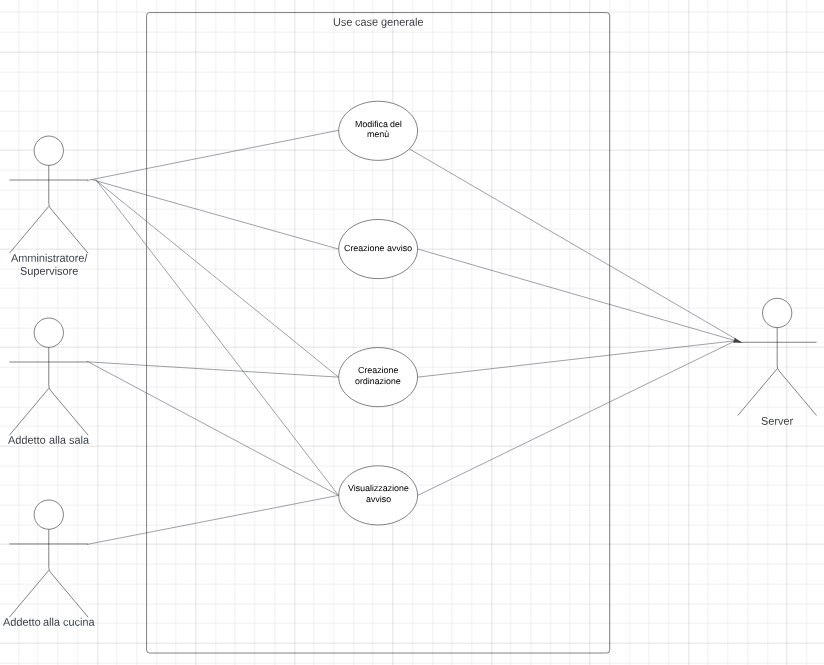
\includegraphics[scale=0.8]{img/use_case/use_case_generale.png}
\end{center}

\subsubsection{Creazione piatto}
La creazione del piatto è una delle funzionalità più elaborate, in quanto, non basterà essere un amministratore/supervisore e inserire i dati (nome, descrizione, allergeni, categoria e prezzo) necessari alla creazione di un piatto. Verrà infatti controllata l'esistenza del piatto e, nel caso di esito positivo il piatto non verrà creato, altrimenti verrà aggiunto alla categoria selezionata.
\begin{center}
  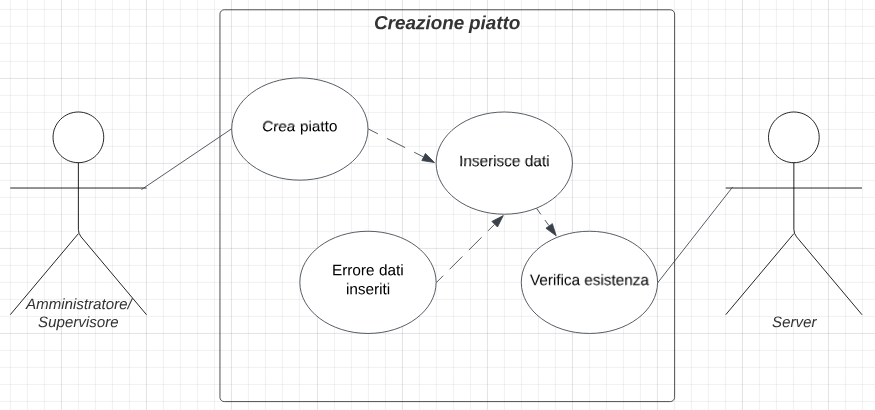
\includegraphics[scale=0.65]{img/use_case/use_case-creazione_piatto.png}
\end{center}
\subsubsection{Eliminazione piatto}
L'eliminazione del piatto è tutto sommato una funzionalità semplice ed autoesplicativa. Viene semplicemente scelto, da un amministratore/supervisore, il piatto che si desidera eliminare, una volta eliminato ci sarà una richiesta di conferma di eliminazione.
\begin{center}
  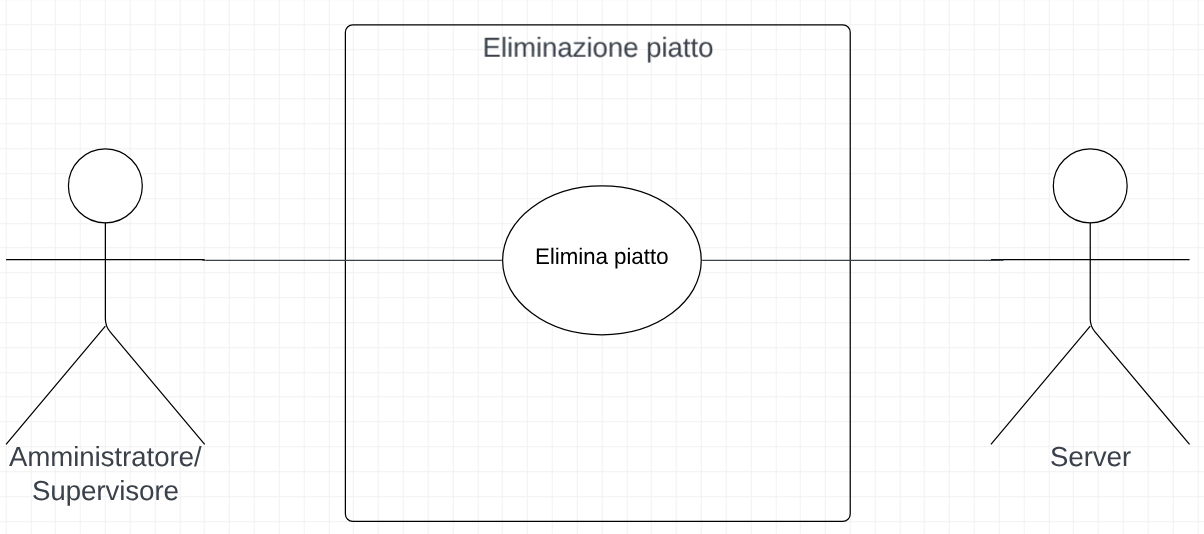
\includegraphics[scale=0.5]{img/use_case/use_case-eliminazione_piatto.png}
\end{center}
\newpage
\subsubsection{Creazione ordinazione}
La creazione di un ordinazione è un requistio fondamentale per la corretta gestione di un'attività di ristorazione che sia essa una tavola calda, un Autogrill o un classico risotrante. Per prima cosa è necessario che l'utente registrato che prova a creare un ordinazione è un "addetto alla sala". Infatti nel caso in cui l'utente registrato non appartiene a questa categoria, non gli sarà permesso a priori la creazione di un ordinazione. Per creare un ordinazione è necessario scegliere un tavolo (tramite l'identificativo associato), e selezionare i piatti che si vogliono aggiungere all'ordinazione (sarà possibile registrare più ordinazioni per lo stesso tavolo in momenti separati).
\begin{center}
  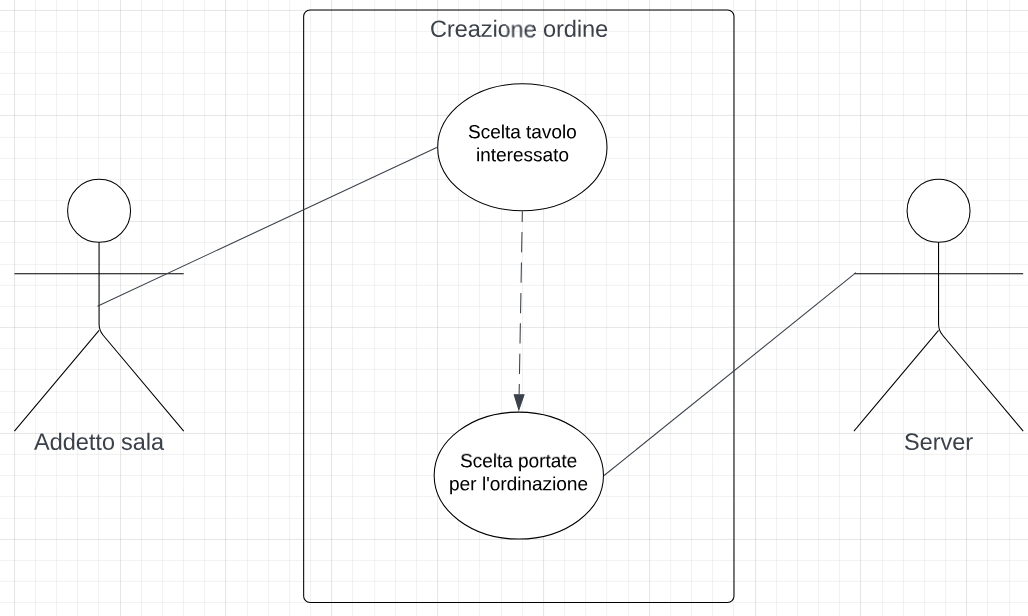
\includegraphics[scale=0.6]{img/use_case/use_case-creazione_ordine.png}
\end{center}
\newpage
\subsubsection{Creazione notifica}
La creazione di un avviso (notifica), è un aspetto fondamentale del software in quanto permette all'amministratore/supervisore di comunicare informazioni importanti indistintamente ad ogni utente. Infatti gli unici utenti con permessi per creare un avviso (notifica) sono proprio l'amministratore e i supervisori.
\begin{center}
  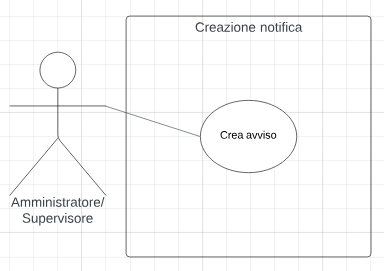
\includegraphics[scale=0.6]{img/use_case/use_case-creazione_notifica.png}
\end{center}
\newpage
\subsection{Tabelle cockburn}
Ci è stato richiesto di presentare, tra i casi d'uso assegnati, quattro casi
specifici a scelta descrivendoli tramite \textbf{tabelle di Cockburn}.
\paragraph{Cosa sono?} Le tabelle di Cockburn (create da \textit{Alistair Cockburn}, dal quale prendono il nome) sono un formalismo di rappresentazione dei casi d'uso.\\
La politica adotta la rappresentazione di un Main scenario nella quale uno o più attori interagiscono
tra loro attraverso l'invocazione di trigger e descrivendo (in formato tabellare) gli eventi.
\\
\\Per garantire una certa corenza al committente e una comprensione a tutto tondo abbiamo scelto gli stessi casi esplorati nella presentazione dei casi d'uso.
\subsubsection{Creazione Ordinazione}
\begin{table}[H]
  \def\arraystretch{1.5}
  \begin{tabularx}{\linewidth}{|l|X|X|X|}
    \hline \textbf{Use Case \#1}           & \multicolumn{3} {l|}{\textbf{Creazione ordinazione}}                                                                                                      \\ \hline \textbf{Goal in
    Context}                               & \multicolumn{3}{>{\hsize=\dimexpr 3\hsize+4\tabcolsep+2\arrayrulewidth\relax}X|}{                                                                         %
    L'addetto alla sala vuole creare una nuova ordinazione per un tavolo}                                                                                                                              \\
    \hline \textbf{Preconditions}          &
    \multicolumn{3}{l|}{L'addetto alla sala deve essersi autenticato correttamente}                                                                                                                    \\
    \hline \textbf{Success End Conditions} &
    \multicolumn{3}{l|}{La nuova ordinazione è stata creata}                                                                                                                                           \\
    \hline \textbf{Failed End Conditions}  &
    \multicolumn{3}{l|}{Le informazioni inserite non sono valide}                                                                                                                                      \\
    \hline \textbf{Primary Actor}          &
    \multicolumn{3}{l|}{Utente autenticato}                                                                                                                                                            \\
    \hline \textbf{Trigger}                & \multicolumn{3}{l|}{Pressione del tasto "crea ordinazione"}                                                                                               \\

    \hline \multirow{2}{*}{\textbf{Description}}
                                           & \textbf{Step}                                                                     & \textbf{Addetto sala}        & \textbf{Server}                        \\
    \cline{2-4}                            & 1                                                                                 & Sceglie il tavolo            &                                        \\
    \cline{2-4}                            & 2                                                                                 & Sceglie i piatti da inserire &                                        \\
    \cline{2-4}                            & 3                                                                                 & Conferma l'ordine            & Verifica esistenza del tavolo          \\
    \cline{2-4}                            & 4                                                                                 &                              & Verifica esistenza dei piatti inseriti \\

    \cline{2-4}                            & 5                                                                                 &                              & Registra ordine                        \\
    \hline
  \end{tabularx}
\end{table}
\subsubsection{Eliminazione piatto}
\begin{table}[H]
  \def\arraystretch{1.5}
  \begin{tabularx}{\linewidth}{|l|X|X|X|}
    \hline \textbf{Use Case \#2}                 & \multicolumn{3} {l|}{\textbf{Eliminazione piatto}}                                                                                       \\ \hline \textbf{Goal in
    Context}                                     & \multicolumn{3}{>{\hsize=\dimexpr 3\hsize+4\tabcolsep+2\arrayrulewidth\relax}X|}{                                                        %
    L'utente vuole eliminare un piatto dal menù}                                                                                                                                            \\
    \hline \textbf{Preconditions}                &
    \multicolumn{3}{l|}{L'utente è autenticato correttamente ed ha i permessi}                                                                                                              \\
    \hline \textbf{Success End Conditions}       &
    \multicolumn{3}{l|}{Il piatto è stato eliminato}                                                                                                                                        \\
    \hline \textbf{Failed End Conditions}        &
    \multicolumn{3}{l|}{Il piatto che ha provato ad eliminare non è valido}                                                                                                                 \\
    \hline \textbf{Primary Actor}                &
    \multicolumn{3}{l|}{Amministratore/supervisore}                                                                                                                                         \\
    \hline \textbf{Trigger}                      & \multicolumn{3}{l|}{Pressione tasto "elimina piatto"}                                                                                    \\

    \hline \multirow{2}{*}{\textbf{Description}} & \textbf{Step}                                                                     &
    \textbf{Client}                              & \textbf{Server}                                                                                                                          \\
    \cline{2-4}                                  & 1                                                                                 & Seleziona il piatto da eliminare &                   \\
    \cline{2-4}                                  & 2                                                                                 & Apertura dialog di conferma      &                   \\
    \cline{2-4}                                  & 3                                                                                 & Conferma l'eliminazione          &                   \\
    \cline{2-4}                                  & 4                                                                                 &                                  & Elimina il piatto \\
    \hline
  \end{tabularx}
\end{table}

\subsubsection{Creazione piatto}
\begin{table}[H]
  \def\arraystretch{1.5}
  \begin{tabularx}{\linewidth}{|l|X|X|X|}
    \hline \textbf{Use Case \#3}                 & \multicolumn{3} {l|}{\textbf{Creazione piatto}}                                                                                                                                                                                            \\ \hline \textbf{Goal in
    Context}                                     & \multicolumn{3}{>{\hsize=\dimexpr 3\hsize+4\tabcolsep+2\arrayrulewidth\relax}X|}{L'utente vuole creare un piatto da aggiungere al menù}                                                                                                    \\
    \hline \textbf{Preconditions}                &
    \multicolumn{3}{l|}{L'utente è collegato correttamente ed ha i permessi necessari}                                                                                                                                                                                                        \\
    \hline \textbf{Success End Conditions}       &
    \multicolumn{3}{l|}{Il piatto è stato creato}                                                                                                                                                                                                                                             \\
    \hline \textbf{Failed End Conditions}        &
    \multicolumn{3}{l|}{Le informazioni inserite sono già presenti o non valide}                                                                                                                                                                                                              \\
    \hline \textbf{Primary Actor}                &
    \multicolumn{3}{l|}{Amministratore/supervisore}                                                                                                                                                                                                                                           \\
    \hline \textbf{Trigger}                      & \multicolumn{3}{l|}{Apertura schermata creazione piatto}                                                                                                                                                                                   \\

    \hline \multirow{2}{*}{\textbf{Description}} & \textbf{Step}                                                                                                                           &
    \textbf{Client}                              & \textbf{Server}                                                                                                                                                                                                                            \\
    \cline{2-4}                                  & 1                                                                                                                                       & Inserisce i dati richiesti per la creazione &                                                    \\
    \cline{2-4}                                  & 2                                                                                                                                       & Clicca tasto "crea piatto"                  &                                                    \\
    \cline{2-4}                                  & 3                                                                                                                                       &                                             & Verifica la possibilità della creazione del piatto \\
    \cline{2-4}                                  & 4                                                                                                                                       &                                             & Salva il piatto                                    \\
    \hline
  \end{tabularx}
\end{table}
\subsubsection{Creazione notifica}
\begin{table}[H]
  \def\arraystretch{1.5}
  \begin{tabularx}{\linewidth}{|l|X|X|X|}
    \hline \textbf{Use Case \#4}                 & \multicolumn{3} {l|}{\textbf{Creazione notifica}}                                                                                                                           \\ \hline \textbf{Goal in
    Context}                                     & \multicolumn{3}{>{\hsize=\dimexpr 3\hsize+4\tabcolsep+2\arrayrulewidth\relax}X|}{                                                                                           %
    L'utente vuole creare una notifica da inviare ai dipendenti}                                                                                                                                                               \\
    \hline \textbf{Preconditions}                &
    \multicolumn{3}{l|}{L'utente è autenticato correttamente ed ha i permessi}                                                                                                                                                 \\
    \hline \textbf{Success End Conditions}       &
    \multicolumn{3}{l|}{La notifica è stata creata}                                                                                                                                                                            \\
    \hline \textbf{Failed End Conditions}        &
    \multicolumn{3}{l|}{La notifica con la stessa data è già presente}                                                                                                                                                         \\
    \hline \textbf{Primary Actor}                &
    \multicolumn{3}{l|}{Amministratore/supervisore}                                                                                                                                                                            \\
    \hline \textbf{Trigger}                      & \multicolumn{3}{l|}{Pressione tasto "crea notifica"}                                                                                                                        \\

    \hline \multirow{2}{*}{\textbf{Description}} & \textbf{Step}                                                                     &
    \textbf{Client}                              & \textbf{Server}                                                                                                                                                             \\
    \cline{2-4}                                  & 1                                                                                 & Inserisce titolo e testo della notifica    &                                            \\
    \cline{2-4}                                  & 2                                                                                 & Preme il tasto per confermare la creazione & Verifica se la notifica non è già presente \\
    \cline{2-4}                                  & 3                                                                                 &                                            & Salva la notifica                          \\
    \hline
  \end{tabularx}

\end{table}
\newpage
\subsection{Mock-Up}
Un mock-up , è una realizzazione a scopo illustrativo o meramente espositivo, di un oggetto o un sistema, senza le complete funzioni
dell'originale; un mockup può rappresentare la totalità o solo una parte dell'originale di riferimento (già esistente o in fase di progetto), essere in scala
reale oppure variata.
\begin{center}
  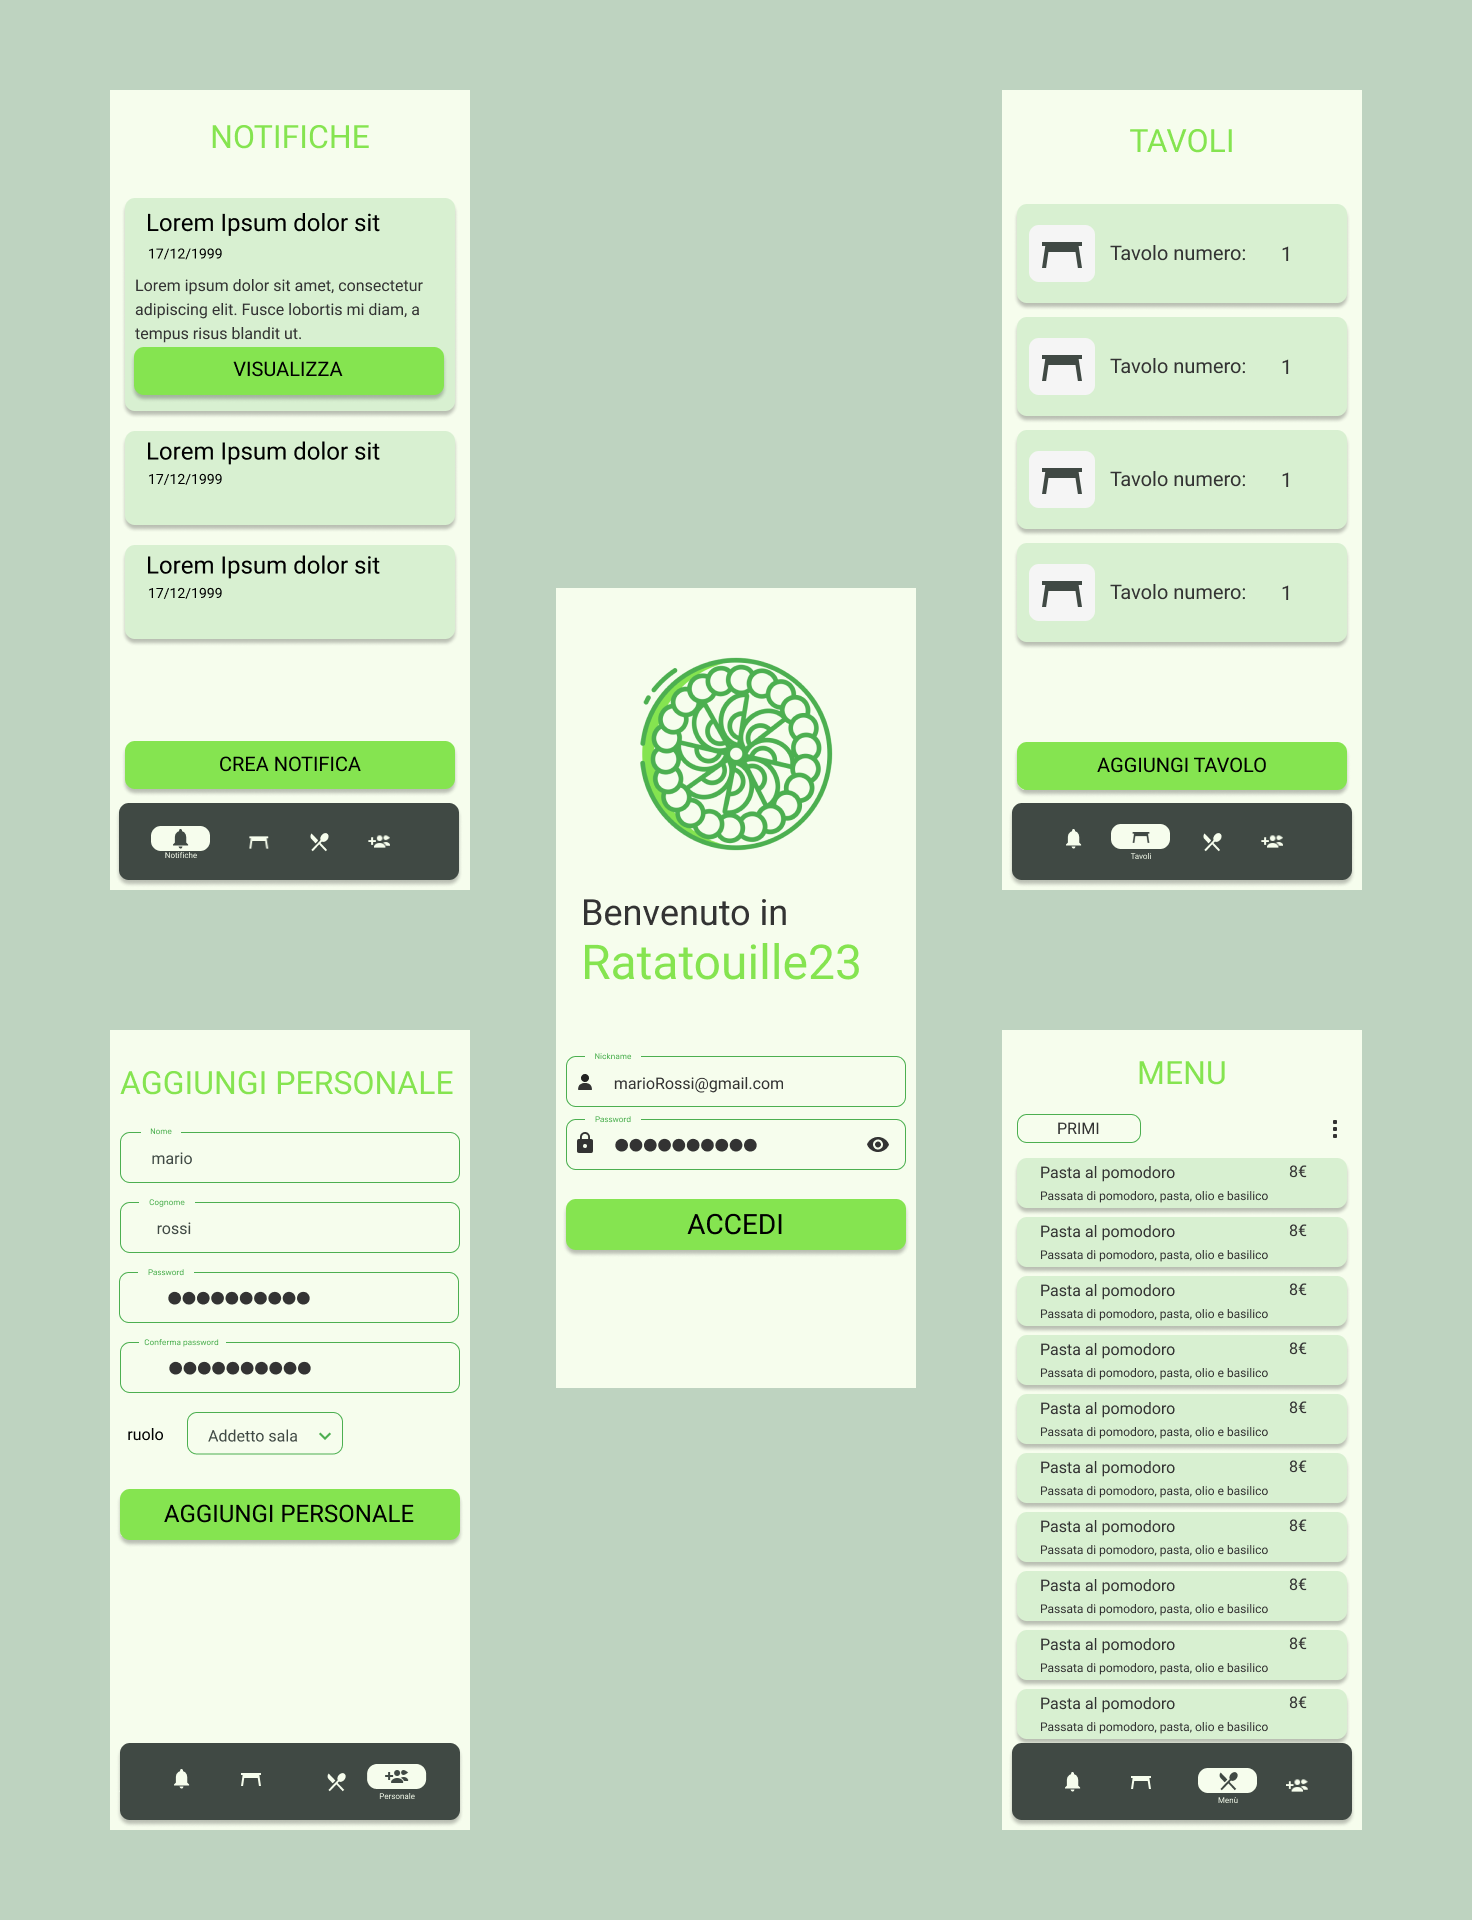
\includegraphics[scale=0.2]{img/Mock-up.doc}
\end{center}
La versione del mock-up qui sopra rappresenta le schermate principali dell'applicazione. Nella realizzazione di quest'applicazione c'è stato uno studio del colore e dell'usabilità, con una palette creata appositamente per non stancare gli occhi e rendere il tutto più "vicino" al cibo possibile.\\
Di seguito andremo a visualizzare i mock-up dei metodi scelti dal team.
\subsubsection{Creazione piatto}
\subsubsection{Eliminazione piatto}
\subsubsection{Creazione ordinazione}
\subsubsection{Creazione notifica}
\section{Specifica dei casi d'uso}
In questa sezione si analizzeranno le classi e come sono relazionate tra loro, daremo un'occhiata ai sequence diagram (in particolare quelli riguardanti due funzionalità dell'applicazione) e agli statechart relativi all'interfaccia grafica. Per fare ciò utilizzeremo:
\begin{enumerate}
  \item Class diagram.
  \item Sequence diagram.
  \item State chart
\end{enumerate}
\subsection{Classi, oggetti e relazioni di analisi}
In questa sezione utilizzeremo i \textit{class diagram} per farci un idea della relazione tra le classi, prima di tutto diamo uno sguardo alla struttura generale che abbiamo creato in fase di analisi:
\begin{figure}[H]
  \centering
  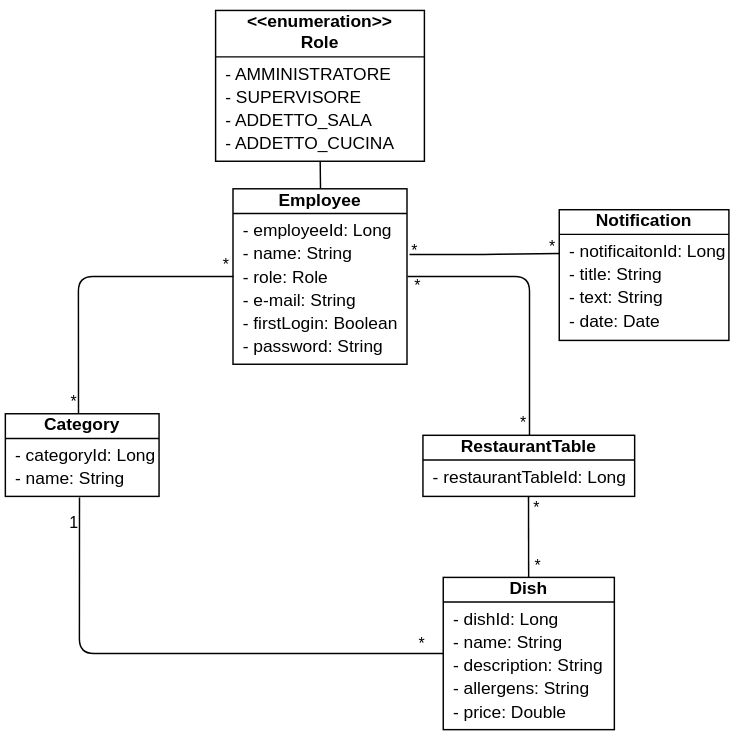
\includegraphics[scale=0.6]{img/class_diagrams/generalClassDiagram.png}
  \caption{Class diagram delle entità}
\end{figure}
D'ora in poi invece, i \textit{class diagram} mostrati, saranno quelli delle funzionalità che sono state assegnate al team di sviluppo.
\newpage
\subsection{Class diagram di analisi - Gestione menù}
In questo class diagram viene analizzato il punto 3 della traccia ovvero la gestione del menù.
\begin{figure}[H]
  \centering
  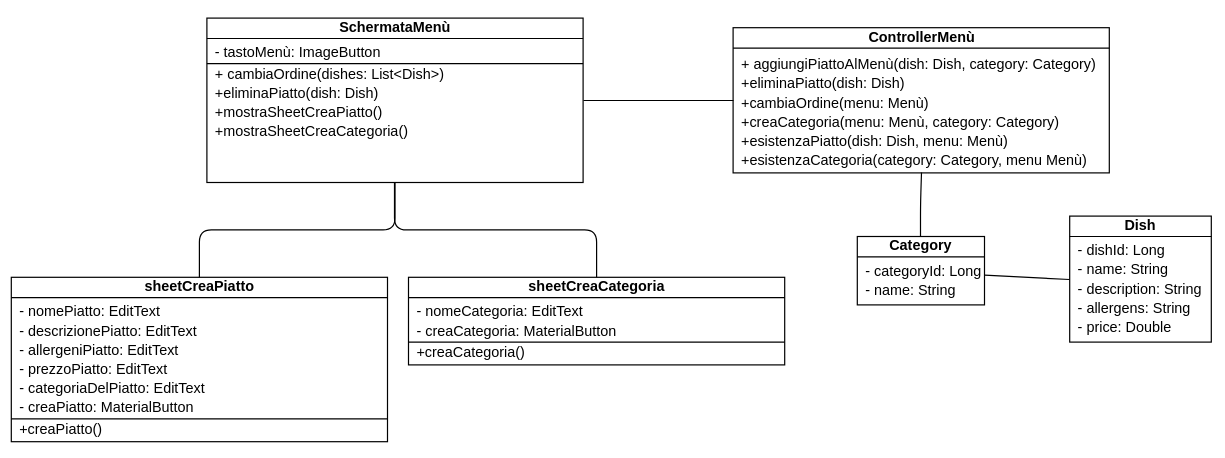
\includegraphics[scale=0.55]{img/class_diagrams/gestioneMenu_class_diagram.png}
  \caption{Class diagram della gestione del menù}
\end{figure}
\newpage
\subsubsection{Class diagram - Creazione utenza}
Nel seguente class diagram verrà analizzato il punto 1, quello nel quale si richiede la creazione di un utente e l'eventuale cambio password nel caso in cui si tratti del primo login, il cambio password verrà però affrontato in un \textit{class diagram} successivo, in modo da poter comprendere anche l'accesso alla piattaforma.

\begin{figure}[H]
  \centering
  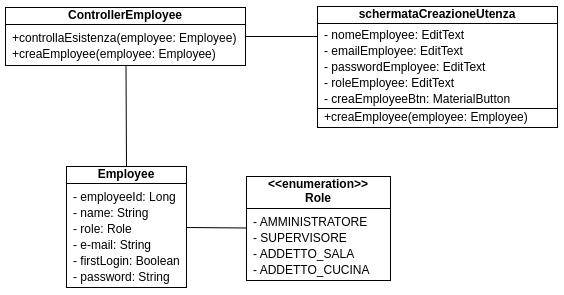
\includegraphics[scale=0.75]{img/class_diagrams/creazioneUtenza_class_diagram.png}
  \caption{Class diagram per la creazione utenze}
\end{figure}
\subsubsection{Class diagram - Accesso alla piattaforma}
Adesso, come detto in precedenza, analizzeremo l'accesso (con conseguente cambio password) alla piattaforma.
\begin{figure}[H]
  \centering
  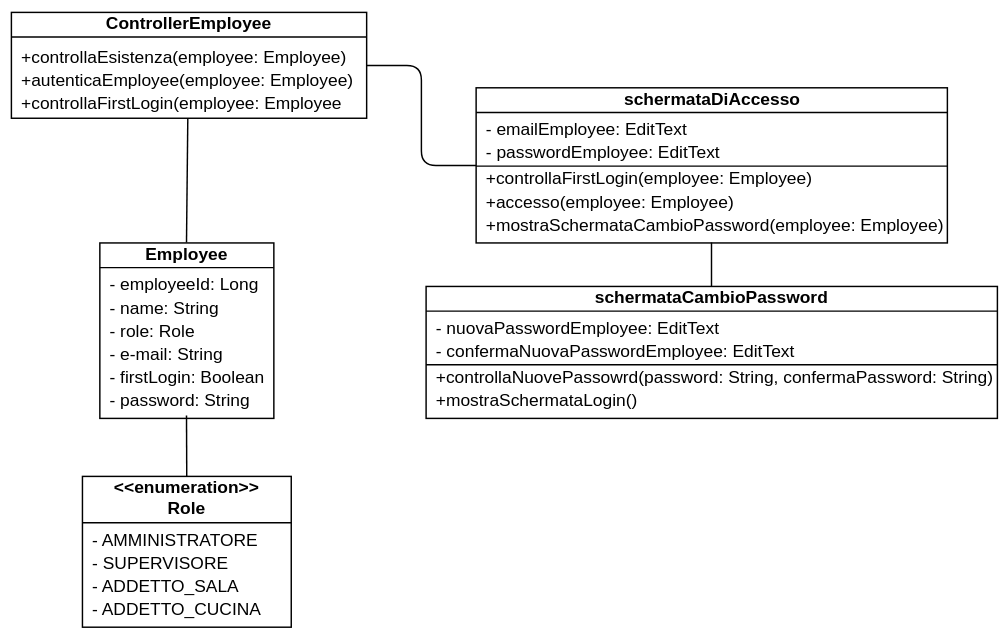
\includegraphics[scale=0.5]{img/class_diagrams/accessoCambioPassword_class_diagram.png}
  \caption{Class diagram dell'accesso alla piattaforma}
\end{figure}
\subsubsection{Class diagram - Gestione tavoli}
Il seguente \textit{class diagram} analizza il punto 6, quindi creazione ordinazioni indicando l'identificativo del tavolo e gli elementi del menù da aggiungere al tavolo.
\begin{figure}[H]
  \centering
  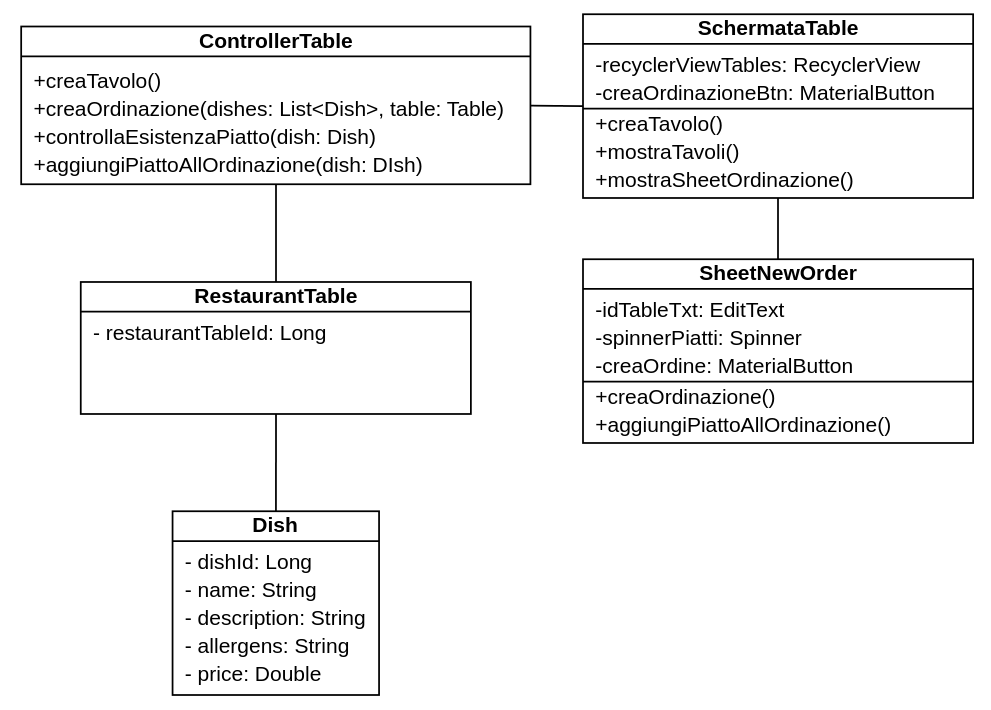
\includegraphics[scale=0.5]{img/class_diagrams/gestioneTavoli_class_diagram.png}
  \caption{Class diagram della gestione dei tavoli}
\end{figure}
\newpage
\subsubsection{Class diagram - Gestione notifiche}
Il seguente \textit{class diagram} analizza il punto 13, quindi creazione di avvisi (notifiche), al quale verrà aggiunta la visualizzazione delle notifiche.
\begin{figure}[H]
  \centering
  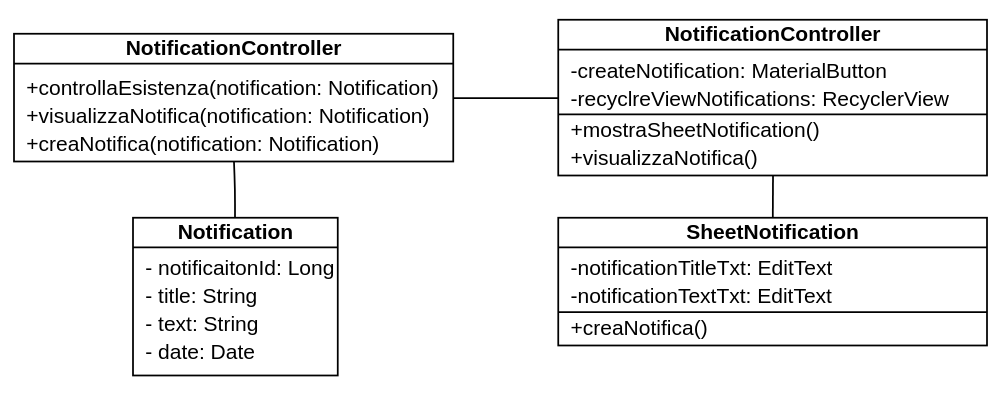
\includegraphics[scale=0.5]{img/class_diagrams/gestioneNotifiche_class_diagram.png}
  \caption{Class diagram della gestione delle notifiche}
\end{figure}
\newpage
\subsection{Sequence diagram}
In questa sezione verranno analizzati due casi d'uso ritenuti fondamentali per questo progetto, in particolare analizzeremo la \textbf{creazione di un piatto}, in quanto parte fondamentale per la gestione di un'attività di ristorazione e la \textbf{gestione delle notifiche}, quest'ultima è stata scelta poiché tutti i dipendenti possono ricevere e visualizzare notifiche ed è fondamentale ai fini del corretto svolgimento dell'attività.
\subsubsection{Sequence diagram - Creazione piatto}
In questo \textit{sequence diagram} l'attore è un superivsore o l'amministratore, sono gli unici due ruoli con i permessi per la creazione di un piatto. I controlli che verranno fatti saranno sull'esistenza della categoria selezionata, verrà controllato se il piatto è già presente ed eventualmente se uno o più campi sono vuoti o non validi.
\begin{figure}[H]
  \centering
  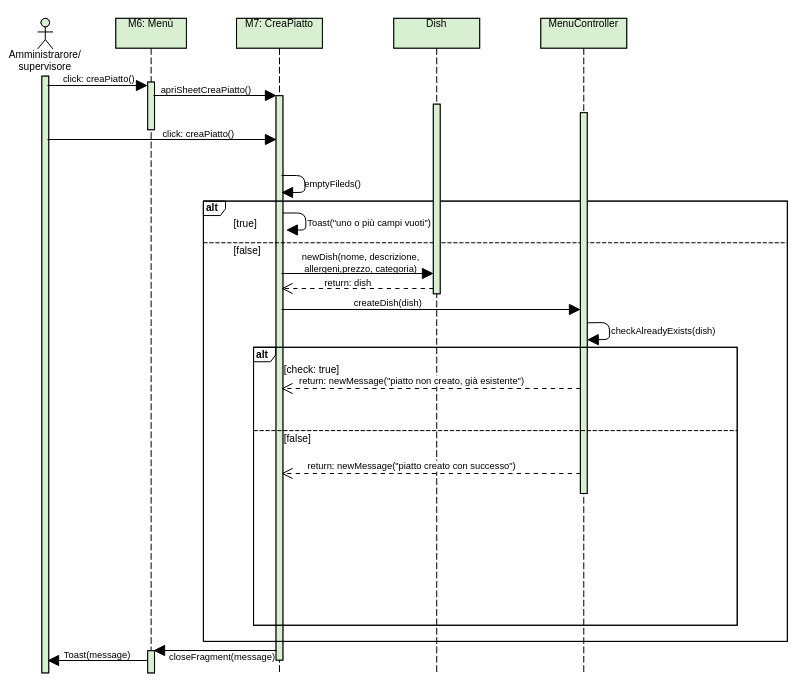
\includegraphics[scale=0.8]{img/sequence/creazionePiatto_sequence_diagram.png}
  \caption{Sequence diagram della creazione di un piatto}
\end{figure}

\subsubsection{Sequence diagram - Creazione piatto}
In questo \textit{sequence diagram} l'attore è un superivsore o l'amministratore, sono gli unici due ruoli con i permessi per la creazione di un piatto. I controlli che verranno fatti saranno sull'esistenza della categoria selezionata, verrà controllato se il piatto è già presente ed eventualmente se uno o più campi sono vuoti o non validi.
\begin{figure}[H]
  \centering
  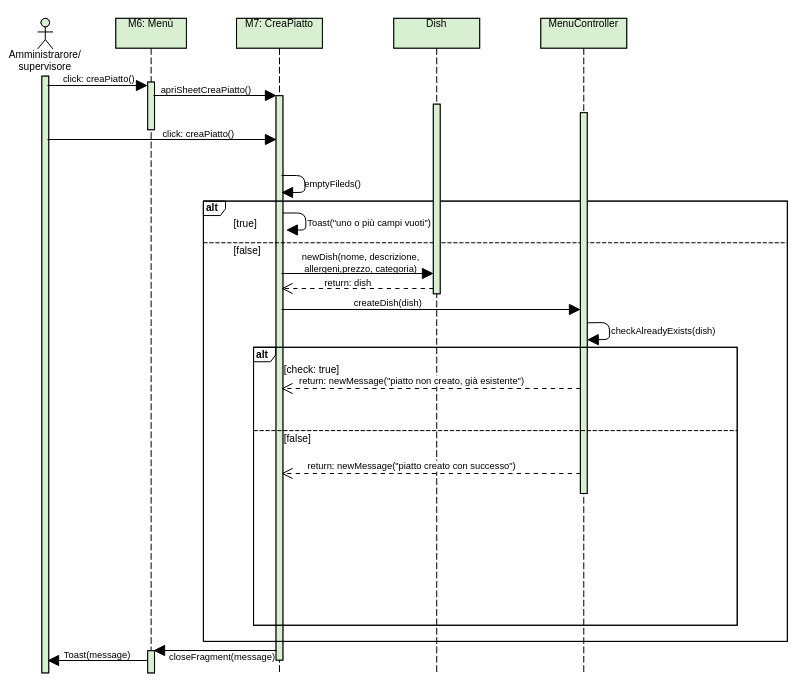
\includegraphics[scale=0.8]{img/sequence/creazionePiatto_sequence_diagram.png}
  \caption{Sequence diagram della creazione di un piatto}
\end{figure}  
\newpage
\subsubsection{Sequence diagram - Creazione notifica}
In questo \textit{sequence diagram} l'attore è un superivsore o l'amministratore, sono gli unici due ruoli con i permessi per la creazione di una. I controlli che verranno eseguiti saranno sull'esistenza della notifica, ed eventualmente se uno o più campi sono vuoti o non validi, in entrambi casi se la notifica verrà valutata "non valida", il sistema farà apparire a schermo un messaggio con scritto "errore nella creazione della notifica".
\begin{figure}[H]
  \centering
  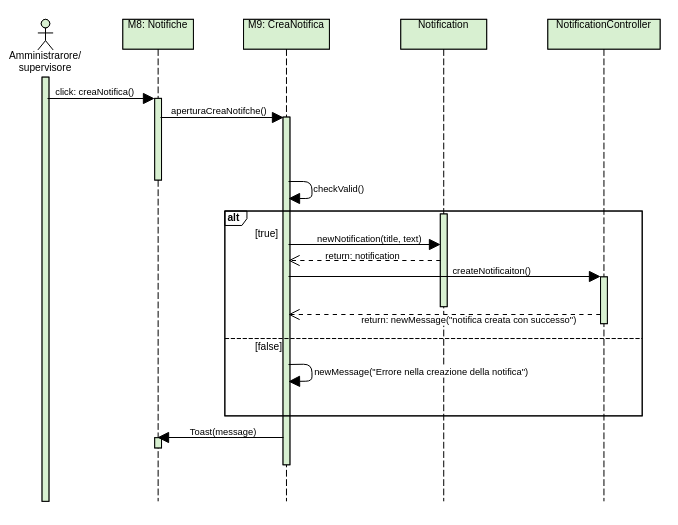
\includegraphics[scale=0.9]{img/sequence/creazioneNotifica_sequence_diagraem.png}
  \caption{Sequence diagram della creazione di una notifica}
\end{figure}  
\newpage
\subsection{State chart}
\end{document}